\chap{复平面}
\section{介绍}
某些学科的历史读起来往往令人兴奋,尤其是在对年代或现有技术存在争议的时候。澄清谁在别人之前做了某件事是历史学家的工作,他们可以帮助理清谁应该为某件事受到指责,谁应该居功。从期刊、书籍和私人信件中理清事件,并将它们置于一个公正的时间序列中,需要学科知识、毅力和客观分析。

对于大多数研究学科,两个日期在确定优先级方面非常重要:论文提交发表的日期,以及被接受的论文发表的日期。这样的协议似乎是一个公平的方案,但无论如何,假设有一个有效的邮政系统,一个公正的同行审查系统,以及许多其他东西。

在数学和科学领域,一些研究人员并不总是有信心将一个萌芽阶段的想法发表出来,如果没有发表,这个想法要么留在他们的脑海里,要么留在他们的桌子上的笔记本上,在研究人员去世后,这些想法可能会被发现,也可能不会被发现。不幸的是,对于研究人员来说,人类的头部并不是一个方便的历史学家的信息宝库!

有时,数学论文出现在与其他学科相关的期刊上,这是可以理解的,不一定受到数学界的监控。同样,历史学家或求知欲强的学者的聪明的侦探工作,将优先权、归因等复杂问题浮出水面,在某些情况下,还有令人讨厌的剽窃嫌疑。

复平面的发明是一个完美的例子,说明当发表数学思想的官方渠道被忽视时,对发明者来说,事情会变得多么糟糕。让我们看看发生了什么。

\section{一点历史}
这一切都始于1813年,当时业余爱好者,瑞士数学家Jean-Robert Argand(1768-1822),在他私人资助的一本“小册子”中发表了他关于复数几何解释的想法:论文探讨了在几何结构中表示虚量的方法[6]\footnote{Essai sur une manière de représenter les quantités imaginaires dans les constructions géométriques}。

这本小册子没有广泛分发,更糟糕的是,它没有写Argand的名字!以一种非常迂回的方式,这本小册子的内容最终被发现,1813年,Jacques Français在一篇论文中重新发表了复平面的思想,并要求原始思想的匿名作者透露自己的身份。Argand站出来,并因他的发明而受到赞扬,今天这个复杂的平面被称为Argand图。。Argand作品的第二版于1874年由出版商Gauthier-Villars[7]出版。

Argand和当时的所有人都不知道,一位挪威测量员卡斯帕·韦塞尔(Caspar Wessel,1745-1818)一直在对丹麦进行三角测量,并开发了数学技术来简化他的工作。其中一个想法是矢量相加的最初想法,另一个是复数的几何解释。

1797年,韦塞尔在丹麦皇家科学院的一次会议上发表了他的第一篇也是唯一一篇描述他的复平面的数学论文,并于1799年在皇家科学院的Mémoires上发表。韦塞尔的论文在数学界隐藏了近一个世纪,直到1895年才被丹麦数学家苏弗斯·克里斯蒂安·朱尔(Sophus Christian Juel, 1855-1935)发现。然而,尽管现在每个人都同意韦塞尔是第一个发明复平面的人,它仍然以Argand的名字命名。

但这并没有结束!苏格兰数学家彼得·格思里·泰特(Peter Guthrie Tait, 1831 - 1901)在他的著作《四元数概论》[21]中写道:

\begin{CJK}{UTF8}{gkai}
    "Wallis,在十七世纪末,建议通过构造一条线来表示一元二次方程的不可能的根,如果它们是真实的,它们就会被放在这条线上。
    他的构造相当于把$sqrt{-1}$看作是一条垂直于测量实数的有向单位线。"
\end{CJK}

John Wallis(1616-1703),是一位天才的英国数学家[22],人们相信Argand、沃Warren和其他人扩展了Wallis和De Moivre的结果,他们在复平面上做了一些早期的工作。

\section{复平面}
与复数发展有关的人之一是杰出的瑞士数学家Leonhard Euler(1707-1783)。Euler证明了恒等式
$$
e^{i \theta}=\cos \theta+i \sin \theta
$$
当$\theta=\pi$时,数学中最美丽的公式之一就出现了:
$$
e^{i \pi}=-1
$$
或
$$
e^{i \pi}+1=0
$$

\begin{figure}[h!]
    \centering
    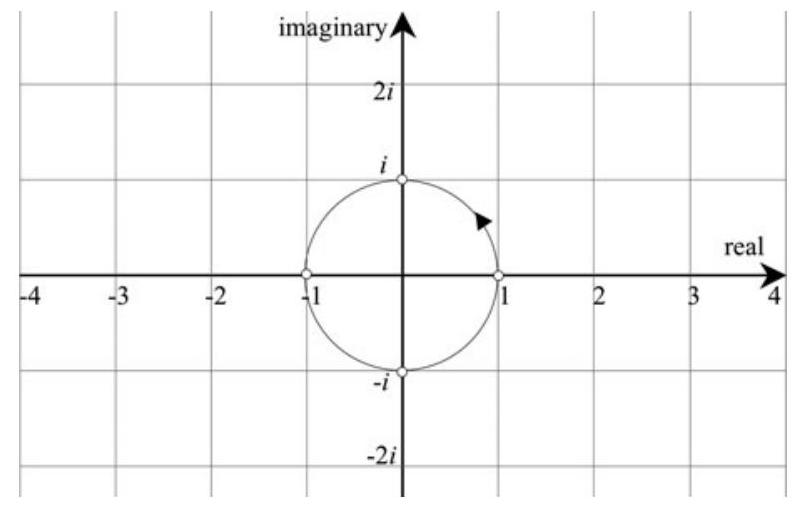
\includegraphics[max width=0.6\textwidth]{2023_01_16_a848224efad29cd66460g-050}
    \caption{带单位圆的复平面}
\end{figure}
它集成了5个重要常数:$0,1,e, \pi$和$i$,以及基本的算术运算:加法,乘法和求幂。

当$\theta=\pi / 2$时,这个公式会产生另一个结果:
$$
e^{i \pi / 2}=\cos \frac{\pi}{2}+i \sin \frac{\pi}{2}=i
$$
因此,\footnote{译者注,和网友讨论,并不止这一种结果,正确的结果应该如此:
\begin{align*}
    \begin{aligned}
        i &=  \cos (\frac{\pi}{2}+2k\pi)+i\sin(\frac{\pi}{2}+2k\pi)\\
        &=e^{i({\pi/2}+2k\pi)},\qquad k\in \mathbb{Z}\\
        i^i &= e^{-(\pi/2+2k\pi)},\qquad k\in \mathbb{Z}\\
    \end{aligned}
\end{align*}

是一个完全的实数的实数幂函数,对应多个值,感谢网友“天津-莲子粥(嵌入式)”。}

$$
\begin{aligned}
i^{i} & =\left(e^{i \pi / 2}\right)^{i} \\
& =e^{i^{2} \pi / 2} \\
& =e^{-\pi / 2} \\
& =0.207879576 \ldots
\end{aligned}
$$
这表明虚数单位自身的幂等于一个实数!\footnote{译者注,参考上一条脚注,应该是一系列实数。}

在第三章中,我们看到虚$i$的幂会产生两个序列$(1,i,-1,-i, 1, \ldots)$和$(1,-i,-1, i, 1, \ldots)$,它们与分别沿逆时针和顺时针方向绕笛卡尔轴旋转时产生的$(x, y,-x,-y, y, x, \ldots)$和$(x,-y,-x, y, x, \ldots)$的模式有着显著的相似之处。这种相似性并非巧合,因为复数属于一个叫做复平面的二维平面,我们现在将描述复平面。

复平面使我们能够可视化复数,横轴记录实数部分,纵轴记录虚数部分,如图4.1所示。该图还显示了一个以单位半径穿过点$1,i,-1,-i$的圆,这是与$i$的幂递增相关的序列。我们可以看到$i^{0}=1, i^{1}=i, i^{2}=-1, i^{3}=-i$和$i^{4}=1$的位置,这表明乘以$i$相当于旋转$90^{\circ}$。为了证明这种旋转效应,图4.2给出了包含四个复数的复平面:
$$
p=2+i, \quad q=-1+2 i, \quad r=-2-i, \quad s=1-2 i
$$
它们之间的距离是$90^{\circ}$。

\begin{figure}[h!]
    \centering
    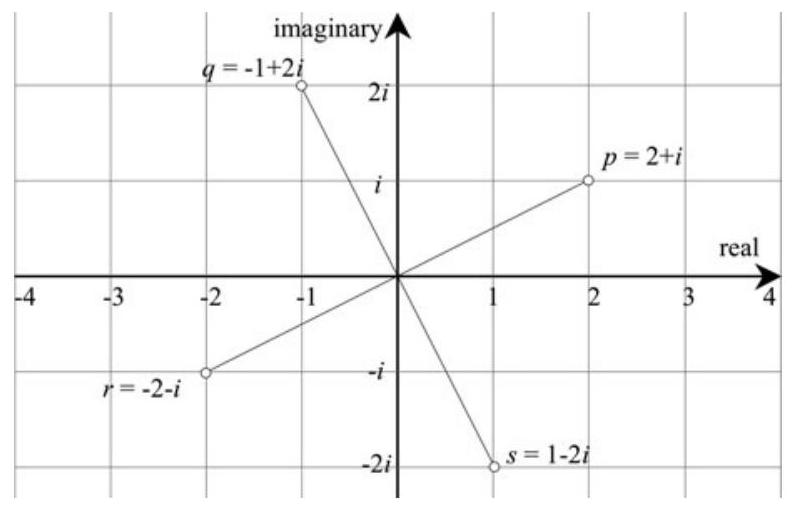
\includegraphics[max width=0.6\textwidth]{2023_01_16_a848224efad29cd66460g-051}
    \caption{标记4个复数的复平面}
\end{figure}

点$p$通过乘以$i$旋转$90^{\circ}$到$q$:
$$
\begin{aligned}
i(2+i) & =2 i+i^{2} \\
& =-1+2 i .
\end{aligned}
$$
点$q$通过乘以$i$旋转$90^{\circ}$到$r$:
$$
\begin{aligned}
i(-1+2 i) & =-i+2 i^{2} \\
& =-2-i .
\end{aligned}
$$
点$r$再乘以$i$旋转$90^{\circ}$到$s$:
$$
\begin{aligned}
i(-2-i) & =-2 i-i^{2} \\
& =1-2 i
\end{aligned}
$$
最后,点$s$乘以$i$被旋转$90^{\circ}$为$p$,:
$$
\begin{aligned}
i(1-2 i) & =i-2 i^{2} \\
& =2+i
\end{aligned}
$$

我们还在第三章中发现,与增加负幂相关的序列:$(1,-i,-1, i, \ldots)$是一个顺时针方向的旋转,这意味着将一个复数除以$i$将它顺时针旋转$90^{\circ}$。然而,我们证明了$i^{-1}=-i$,用$-i$乘以一个复数要比用$i$除以简单得多。所以让我们重复上面的练习来证明这一点。

点$p$乘以$-i$被旋转$-90^{\circ}$到$s$:
$$
\begin{aligned}
-i(2+i) & =-2 i-i^{2} \\
& =1-2 i .
\end{aligned}
$$
点$s$再乘以$-i$旋转$-90^{\circ}$到$r$:
$$
\begin{aligned}
-i(1-2 i) & =-i+2 i^{2} \\
& =-2-i .
\end{aligned}
$$
点$r$再乘以$-i$旋转$-90^{\circ}$到$q$,:
$$
\begin{aligned}
-i(-2-i) & =2 i+i^{2} \\
& =-1+2 i .
\end{aligned}
$$
最后,点$q$乘以$-i$被旋转$-90^{\circ}$为$p$:
$$
\begin{aligned}
-i(-1+2 i) & =i-2 i^{2} \\
& =2+i .
\end{aligned}
$$
因此,将一个复数旋转$\pm 90^{\circ}$,乘以$\pm i$。

在第3章中,我们看到$\sqrt{\pm i}$的根为
$$
\begin{aligned}
& \sqrt{+i}=\pm \frac{\sqrt{2}}{2}(1+i) \\
& \sqrt{-i}=\pm \frac{\sqrt{2}}{2}(1-i)
\end{aligned}
$$
请注意如图4.3所示,每个根之间的距离为$180^{\circ}$,这表明角度与它们的行为有关。例如,$\sqrt{+i}$的正根是$\sqrt{2}/ 2(1+i)$,离实轴为$45^{\circ}$。将这个根乘以它自己,将它$45^{\circ}$旋转到$i$轴。类似地,负根是$-\sqrt{2}/ 2(1+i)$,离实轴为$225^{\circ}$。这个根乘以它自己,将它$225^{\circ}$旋转到$i$轴。$\sqrt{-i}$的根也是如此。

\begin{figure}[h!]
    \centering
    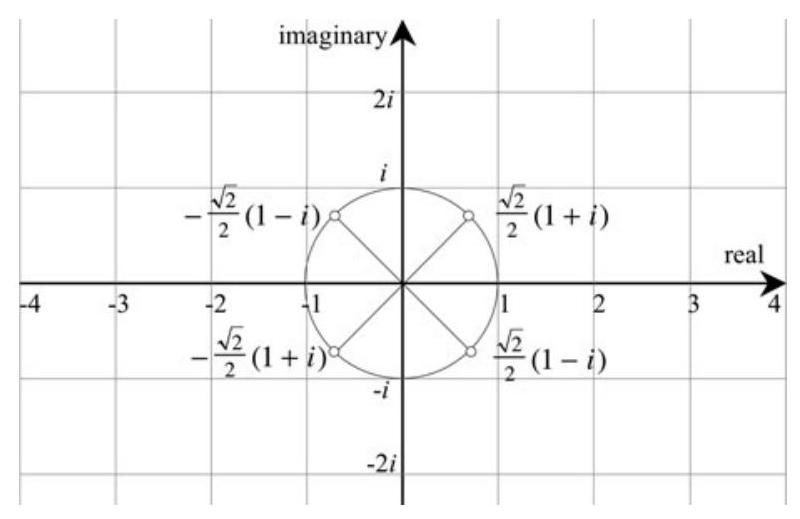
\includegraphics[max width=0.6\textwidth]{2023_01_16_a848224efad29cd66460g-052}
    \caption[short]{$\sqrt{\pm i}$的根}
\end{figure}

这些观察似乎表明,我们可以构造一个能够使另一个复数旋转任意角度的复数。这是真的,我们接下来会讲到。

\section{极坐标表示法}
在复平面上放置一个复数,我们得到极坐标表示,在极坐标表示中,我们从原点到复数形成一条直线,如图4.4所示。这条线的长度是$r$,等于$\sqrt{a^{2}+b^{2}}$,这就是为什么复数的范数是用毕达哥拉斯公式定义的:
\begin{figure}[h!]
    \centering
    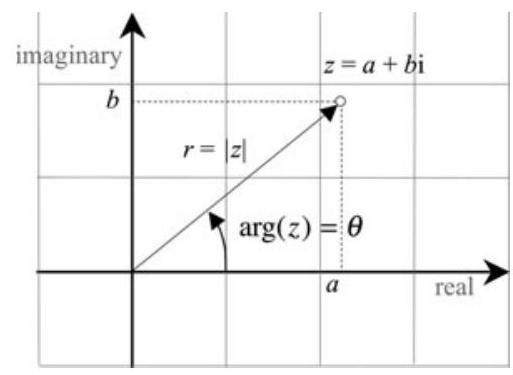
\includegraphics[max width=0.6\textwidth]{2023_01_16_a848224efad29cd66460g-053}
    \caption[short]{复数的极坐标表示
    }
\end{figure}

$$
r=|z|=\sqrt{a^{2}+b^{2}} .
$$
直线与实轴之间的角度$\theta$称为$z$的参数
$$
\arg (z)=\theta
$$
其中
$$
\tan \theta=\frac{b}{a} .
$$
我们计算$\arg (z)$使用
$$
\begin{array}{ll}
\text { 第一象限 } a>0, b>0 & \theta=\arctan (b / a) \\
\text { 第二和第三象限 } a<0 & \theta=\arctan (b / a)+\pi \\
\text { 第四象限 } a>0, b<0 & \theta=\arctan (b / a)+2 \pi .
\end{array}
$$
从图4.4中我们可以看到,z的水平分量是$r \cos \theta$,垂直分量是$r \sin \theta$,这使得我们可以写
$$
\begin{aligned}
z & =a+b i \\
& =r \cos \theta+r i \sin \theta \\
& =r(\cos \theta+i \sin \theta) .
\end{aligned}
$$
如上所述,欧拉的发现之一是关于$e^{\theta}, \sin \theta$和$ cos \theta$幂级数的恒等式:
$$
e^{i \theta}=\cos \theta+i \sin \theta
$$
这允许我们写作
$$
z=r e^{i \theta} .
$$
有了这个发现,我们现在可以用极坐标表示法来重新讨论两个复数的乘积和商。例如,给定下列复数
$$
\begin{aligned}
z & =r e^{i \theta} \\
w & =s e^{i \phi}
\end{aligned}
$$
他们的乘积
$$
\begin{aligned}
z w & =r s e^{i \theta} e^{i \phi} \\
& =r s e^{i(\theta+\phi)} \\
& =r s[\cos (\theta+\phi)+i \sin (\theta+\phi)]
\end{aligned}
$$
所以两个复数的乘积会产生第三个有范数的复数
$$
|z w|=r s
$$
且参数
$$
\arg (z w)=\theta+\phi
$$
这里两个角直接相加了。

接下来,除法:
$$
\begin{aligned}
\frac{z}{w} & =\frac{r e^{i \theta}}{s e^{i \phi}} \\
& =\frac{r}{s} e^{i(\theta-\phi)} \\
& =\frac{r}{s}[\cos (\theta-\phi)+i \sin (\theta-\phi)]
\end{aligned}
$$
其中,范数是
$$
\left|\frac{z}{w}\right|=\frac{r}{s}
$$
且参数为
$$
\arg (z / w)=\theta-\phi
$$
这里是两个角度相减了。

让我们用一个例子来应用这些公式。图$4.5$显示了两个复数
$$
\begin{gathered}
z=2+2 i \\
w=-1+i
\end{gathered}
$$
在极坐标形式里面是
$$
\begin{aligned}
z & =2 \sqrt{2}\left(\cos 45^{\circ}+i \sin 45^{\circ}\right)=2 \sqrt{2} e^{i \pi / 4} \\
w & =\sqrt{2}\left(\cos 135^{\circ}+i \sin 135^{\circ}\right)=\sqrt{2} e^{i 3 \pi / 4} .
\end{aligned}
$$
用普通的复代数,乘积$z w$是
$$
z w=(2+2 i)(-1+i)=-4
$$
\begin{figure}[h!]
    \centering
    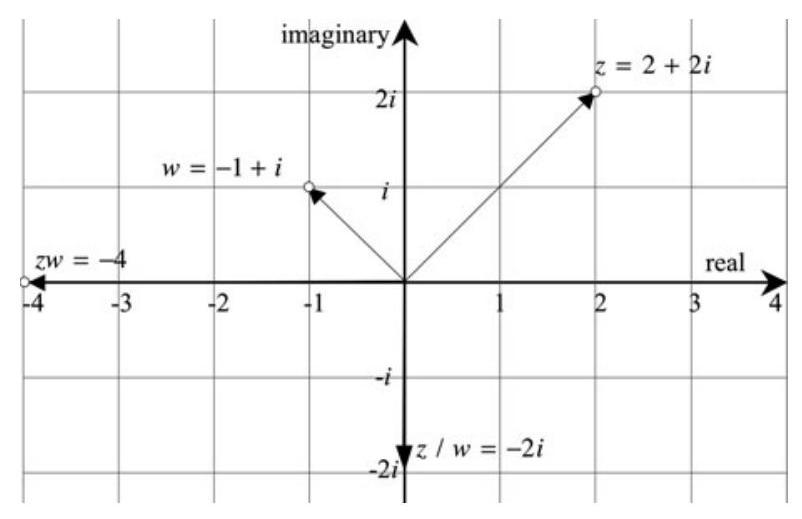
\includegraphics[max width=0.6\textwidth]{2023_01_16_a848224efad29cd66460g-055}
    \caption[short]{两个复数的乘积}
\end{figure}
用极坐标形式是:
$$
\begin{aligned}
|z w| & =2 \sqrt{2} \sqrt{2}=4 \\
\arg (z w) & =45^{\circ}+135^{\circ}=180^{\circ}
\end{aligned}
$$
这里编码为$-4$。

现在让我们用普通的复代数和极坐标形式来计算商$z / w$。
$$
\begin{aligned}
\frac{z}{w} & =\frac{(2+2 i)}{(-1+i)} \frac{(-1-i)}{(-1-i)} \\
& =\frac{-2-2 i-2 i-2 i^{2}}{1+1} \\
& =-2 i
\end{aligned}
$$
接下来,使用极坐标形式:
$$
\begin{aligned}
|z / w| & =\frac{2 \sqrt{2}}{\sqrt{2}}=2 \\
\arg (z / w) & =45^{\circ}-135^{\circ}=-90^{\circ}
\end{aligned}
$$
这编码复数$-2 i$。这些结果如图4.5所示。

我们还可以使用欧拉公式计算$\sqrt{i}$ ,如下所示
$$
e^{i \theta}=\cos \theta+i \sin \theta
$$
将$\theta=\pi / 2$代入
$$
e^{i \pi / 2}=\cos \frac{\pi}{2}+i \sin \frac{\pi}{2}=i
$$
两边同时开根号,得到
$$
\begin{aligned}
e^{i \pi / 4} & =\pm \sqrt{i} \\
\cos \frac{\pi}{4}+i \sin \frac{\pi}{4} & =\pm \sqrt{i} \\
\pm \frac{\sqrt{2}}{2}(1+i) & =\pm \sqrt{i}
\end{aligned}
$$
为了找到$\sqrt{-i}$,我们代入$\theta=-\pi / 2$:
$$
\begin{aligned}
e^{-i \pi / 2} & =\cos \left(-\frac{\pi}{2}\right)+i \sin \left(-\frac{\pi}{2}\right)=-i \\
& =\cos \left(\frac{\pi}{2}\right)-i \sin \left(\frac{\pi}{2}\right)=-i
\end{aligned}
$$
两边同时开根号,得到
$$
\begin{aligned}
e^{-i \pi / 4} & =\pm \sqrt{-i} \\
\cos \left(\frac{\pi}{4}\right)-i \sin \left(\frac{\pi}{4}\right) & =\pm \sqrt{-i} \\
\pm \frac{\sqrt{2}}{2}(1-i) & =\pm \sqrt{-i}
\end{aligned}
$$
用类似的方法可以找到更高次的根。

\section{转子}
极坐标形式说明了这样一个事实:范数为$r$的复数$z=r e^{i \theta}$与范数为$s$的复数$w=s e^{i \phi}$相乘,就得到了第三个范数为$r s$的复数。因此,为了避免缩放$z, w$必须有一个范数单位$1$。在这种情况下,$w$充当转子。例如,用$4+5 i$乘以$1+0 i$,它就没有缩放和旋转。然而,用$4+5 i$乘以$0+i$将它旋转$90^{\circ}$而不进行任何缩放。

因此,要将$2+2 i$旋转$45^{\circ}$,我们必须将它乘以$e^{i \pi / 4}$:
$$
\begin{aligned}
e^{i \pi / 4} & =\cos 45^{\circ}+i \sin 45^{\circ}=\frac{\sqrt{2}}{2}(1+i) \\
\frac{\sqrt{2}}{2}(1+i)(2+2 i) & =\frac{\sqrt{2}}{2} 4 i \\
& =2 \sqrt{2} i .
\end{aligned}
$$
因此$e^{i \theta}$将任何复数旋转一个角度$\theta$。

要使复数$x+y i$旋转一个角度$\theta$,我们可以将它乘以转子$\cos \theta+i \sin \theta$:
$$
\begin{aligned}
x^{\prime}+y^{\prime} i & =(\cos \theta+i \sin \theta)(x+y i) \\
& =x \cos \theta-y \sin \theta+i(x \sin \theta+y \cos \theta)
\end{aligned}
$$
矩阵形式是:
$$
\left[\begin{array}{cc}
x^{\prime} & -y^{\prime} \\
y^{\prime} & x^{\prime}
\end{array}\right]=\left[\begin{array}{cc}
\cos \theta & -\sin \theta \\
\sin \theta & \cos \theta
\end{array}\right]\left[\begin{array}{cc}
x & -y \\
y & x
\end{array}\right] .
$$
在继续之前,让我们考虑转子的复共轭对旋转方向的影响,我们可以通过将$x+y i$乘以转子$\cos \theta -i \sin \theta$来实现
$$
\begin{aligned}
x^{\prime}+y^{\prime} i & =(\cos \theta-i \sin \theta)(x+y i) \\
& =x \cos \theta+y \sin \theta-i(x \sin \theta+y \cos \theta)
\end{aligned}
$$
矩阵形式是
$$
\left[\begin{array}{cc}
x^{\prime} & -y^{\prime} \\
y^{\prime} & x^{\prime}
\end{array}\right]=\left[\begin{array}{cc}
\cos \theta & \sin \theta \\
-\sin \theta & \cos \theta
\end{array}\right]\left[\begin{array}{cc}
x & -y \\
y & x
\end{array}\right]
$$
也就是绕原点旋转$-\theta$。

因此,我们定义一个转子$\mathbf{R}_{\theta}$和它的共轭$\mathbf{R}_{\theta}^{\dagger}$为
$$
\begin{aligned}
& \mathbf{R}_{\theta}=\cos \theta+i \sin \theta \\
& \mathbf{R}_{\theta}^{\dagger}=\cos \theta-i \sin \theta
\end{aligned}
$$
其中$\mathbf {R} _{\theta}$旋转$+ \theta$,和$\mathbf{R}_{\theta}^{\dagger}$旋转$- \theta$。注意,使用了匕首$\dagger$符号。

\section{总结}
在本章中,我们发现了用复平面来表示复数的图形化解释。欧拉公式$e^{i \theta}=\cos \theta+i \sin \theta$允许我们将复数表示为$e$的虚数次幂,从而使我们可以轻松地计算乘积和商。总的来说,这些想法把我们引向了转子的想法,它将使用四元数来开发。

\subsection{运算符总结}
\subsubsection*{复数}
$$
\begin{aligned}
z & =a+b i \\
|z| & =\sqrt{a^{2}+b^{2}}
\end{aligned}
$$

\subsubsection*{极坐标表示}

$$
\begin{aligned}
z & =r e^{i \theta} \\
z & =r(\cos \theta+i \sin \theta) \\
r & =|z| \\
\tan \theta & =b / a \\
\theta & =\arg (z)
\end{aligned}
$$

\begin{align*}
    \begin{aligned}
        &\text{第一象限  } a>0, b>0 && \theta=\arctan (b / a)\\
        &\text{第二和第三象限  } a<0 && \theta=\arctan (b / a)+\pi\\
        &\text{第四象限  } a>0, b<0 && \theta=\arctan (b / a)+2 \pi.
    \end{aligned}
\end{align*}


\subsubsection*{乘积}
$$
\begin{aligned}
z & =r e^{i \theta} \\
w & =s e^{i \phi} \\
z w & =r s e^{i(\theta+\phi)} \\
& =r s[\cos (\theta+\phi)+i \sin (\theta+\phi)]
\end{aligned}
$$

\subsubsection*{商}
$$
\begin{aligned}
\frac{z}{w} & =\frac{r}{s} e^{i(\theta-\phi)} \\
& =\frac{r}{s}[\cos (\theta-\phi)+i \sin (\theta-\phi)]
\end{aligned}
$$

\subsubsection*{转子}
$$
\begin{aligned}
& \mathbf{R}_{\theta}=\cos \theta+i \sin \theta \\
& \mathbf{R}_{\theta}^{\dagger}=\cos \theta-i \sin \theta
\end{aligned}
$$

\section{样例}
下面是一些进一步使用上述思想的示例。在某些情况下,包括测试来确认结果。
\begin{example}
    
    从$1+2 i$开始,将得到的复数乘以$i$四次,并将结果绘制在复平面上。
    
    点$p$通过乘以$i$旋转$90^{\circ}$到$q$:
    $$
    \begin{aligned}
    i(1+2 i) & =i+2 i^{2} \\
    & =-2+i .
    \end{aligned}
    $$
    
    点$q$通过乘以$i$旋转$90^{\circ}$到$r$:
    $$
    \begin{aligned}
    i(-2+i) & =-2 i+i^{2} \\
    & =-1-2 i
    \end{aligned}
    $$
    
    点$r$再乘以$i$旋转$90^{\circ}$到$s$:
    $$
    \begin{aligned}
    i(-1-2 i) & =-i-2 i^{2} \\
    & =2-i .
    \end{aligned}
    $$
    
    最后,点$s$乘以$i$被旋转$90^{\circ}$为$p$:
    $$
    \begin{aligned}
    i(2-i) & =2 i-i^{2} \\
    & =2+i .
    \end{aligned}
    $$
    
    图$4.6$显示了四个被$90^{\circ}$隔开的复数。
    \begin{figure}[h!]
        \centering
        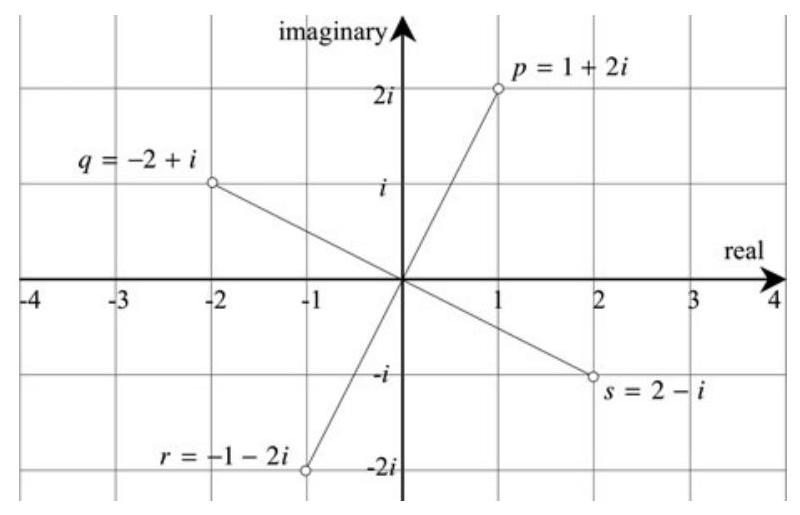
\includegraphics[max width=0.6\textwidth]{2023_01_16_a848224efad29cd66460g-059}
        \caption{有四个复数的复平面}
    \end{figure}
\end{example}

\begin{example}
    用极坐标形式计算乘积$ zw $和商$z / w$。
    $$
    \begin{gathered}
    z=3+3 i \\
    w=-1-i
    \end{gathered}
    $$
    
    乘积:
    $$
    \begin{aligned}
    z & =3 \sqrt{2}\left(\cos 45^{\circ}+i \sin 45^{\circ}\right)=3 \sqrt{2} e^{i \pi / 4} \\
    w & =\sqrt{2}\left(\cos 225^{\circ}+i \sin 225^{\circ}\right)=\sqrt{2} e^{i 5 \pi / 4} \\
    |z w| & =3 \sqrt{2} \sqrt{2}=6 \\
    \arg (z w) & =45^{\circ}+225^{\circ}=270^{\circ}
    \end{aligned}
    $$
    这编码复数$-6 i$。
    
    测试:使用普通的复代数,乘积$ zw $为
    $$
    z w=(3+3 i)(-1-i)=-6 i .
    $$
    
    商:
    $$
    \begin{aligned}
    |z| & =3 \sqrt{2} \\
    |w| & =\sqrt{2} \\
    |z / w| & =3 \sqrt{2} / \sqrt{2}=3 \\
    \arg (z / w) & =45^{\circ}-225^{\circ}=180^{\circ}
    \end{aligned}
    $$
    这编码复数$-3$.
    
    测试:使用普通的复代数,乘积$ z/w $为
    $$
    \begin{aligned}
    \frac{z}{w} & =\frac{(3+3 i)}{(-1-i)} \frac{(-1+i)}{(-1+i)} \\
    & =\frac{-6}{2} \\
    & =-3
    \end{aligned}
    $$
    
    并且符合极坐标形式。
\end{example}

\begin{example}
    设计一个转子,将一个复数旋转$30^{\circ}$而不缩放。
    
    这样开始
    $$
    e^{i \theta}=\cos \theta+i \sin \theta
    $$
    
    令 $\theta=30^{\circ}=\pi / 6$
    $$
    \begin{aligned}
    e^{i \pi / 6} & =\cos 30^{\circ}+i \sin 30^{\circ} \\
    & =\frac{\sqrt{3}}{2}+i \frac{1}{2} \\
    & =\frac{1}{2}(\sqrt{3}+i) .
    \end{aligned}
    $$
    
    测试:让我们用这个转子将$1+0 i$旋转三次到$i$。
    $$
    \begin{aligned}
    \frac{1}{2}(\sqrt{3}+i) \frac{1}{2}(\sqrt{3}+i) \frac{1}{2}(\sqrt{3}+i) 1 & =\frac{1}{8}(\sqrt{3}+i)(\sqrt{3}+i)(\sqrt{3}+i) \\
    & =\frac{1}{8}(2+2 \sqrt{3} i)(\sqrt{3}+i) \\
    & =\frac{1}{8}(2 \sqrt{3}-2 \sqrt{3}+2 i+6 i) \\
    & =i
    \end{aligned}
    $$
\end{example}

\begin{example}
    设计一个转子,将一个复数旋转$-60^{\circ}$而不缩放。
    
    这样开始
    $$
    e^{i \theta}=\cos \theta+i \sin \theta
    $$
    
    令 $\theta=-60^{\circ}=-\pi / 3$
    
    $$
    \begin{aligned}
    e^{-i \pi / 3} & =\cos \left(-60^{\circ}\right)+i \sin \left(-60^{\circ}\right) \\
    & =\frac{1}{2}-\frac{\sqrt{3}}{2} i \\
    & =\frac{1}{2}(1-\sqrt{3} i)
    \end{aligned}
    $$
\end{example}
